
%%%%%%%%% SUMMARY -- 1 page, third person
% e.g:  "The PI will prove" not "I will prove"

%Introduction / Summary (1 page).  The following information is typically included in proposal introductions for this 
%grant. The summary should lead to the proposal body but it should also be a self-contained document, 
%summarizing what is being proposed and why.   
 
% Provide appropriate background that sets the context for the problem and the objectives. 
%State the specific problem (may also be thought of as a need, central research question, or hypothesis) 
%your research will address. 
% State the objectives of the proposed research. 
%State any limits of the proposed research  (may not be needed). 
%Summarize the research methods you will use to achieve research objectives (if clearly covered elsewhere 
%in the introduction, a separate section may not be needed). 


\section{Background}
%this section needs more stats and citations
In the Columbia Basin today, millions of federal dollars are spent on PTAGIS
and other systems to collect environmental data.  This data includes fish
location, ecological community composition, and abiotic data. Yet, the project
results from most research are far from concrete. Despite the lack of
understandable results, important decisions that affect the local environment
and economy have to be made. Decisions like whether or not to conduct major
habitat restoration projects are sometimes made without convincing data to
support them. 

%We should cite something other study / examples in the basin. Foster's talk
% just sticks in my head as a good example
The Columbia Basin is just one small example. Bioinformatics is another 
data intensive field that generates more data that it can process. It is 
%is this 10%? It may be lower
estimated that less than 10\% of the data collected by bioinformatic 
researchers at the University of Idaho actually makes it through processing
\cite{foster}. The rest has to be filtered as best as can be managed, and the 
low value data trimmed out. The problem with 10\% data use is that not just 
the fat, but the meat and bone has to be cut away. Either significantly more
data must be analyzed, or significantly less should be collected. At the very
least, storing the data in an easily readable format can show where the 
gaps are. So far, our experience and research shows similar shortfalls in 
data analysis in the Columbia Basin.

There is a clear need for a tool that simplifies data management.  Specifically,
a tool is needed that allows users to work remotely with data, perform basic manipulations
and filters, visualize data points, and explore data.  We expect that such a
tool would not only simplify the scientific process for researchers with large
data sets, but allow the processing of a larger percentage of relevant data.

\section{Problem Definition}
One of the biggest problems researchers in the Columbia Basin have is moving
their data somewhere meaningful. Central databases like PTAGIS offer a 
central storage and clients can push data there, but they don't offer useful
tools for managing data. Once the data is pushed, it is hard to access and
manipulate. 
Researchers are often in remote locations, and have low bandwidth
connections, but would benefit greatly from a centralized location with 
built-in data management and exploration capabilities.
Creating a robust tool will guarantee ease of use for the data, no matter
the location.

Many researchers have significant data management tasks before even thinking 
about pushing data to the cloud. Once they are ready, they need seamless ways to
synchronize data to and from the cloud. They also need to query their data,
and filter it into small subsets. Most researchers don't have time to learn
new programming languages or interfaces. They need a simple data management tool 
that has an intuitive user 
interface and fits their use cases. Once they
have created a data subset, they will want to share it, save it, copy it, 
and compare it with other data sets. Getting the right data to the right place 
in the right amount of time is crucial.

In this interest, a data management tool needs to be written.  It must meet the
following requirements:

\singlespacing
\begin{itemize}
    \item Provide:
    \begin{itemize}
        \item Reliable data storage
         \item Basic data manipulations
         \item Simple visualizations
     \end{itemize}
     \item Have a gentle learning curve
     \item Allow remote access
     \item Allow local access
     \item Support many data sets (i.e.,  not just PTAGIS data)
 \end{itemize}

 \doublespacing

\section{Objectives}

\begin{figure}[!h]
        \begin{center}
		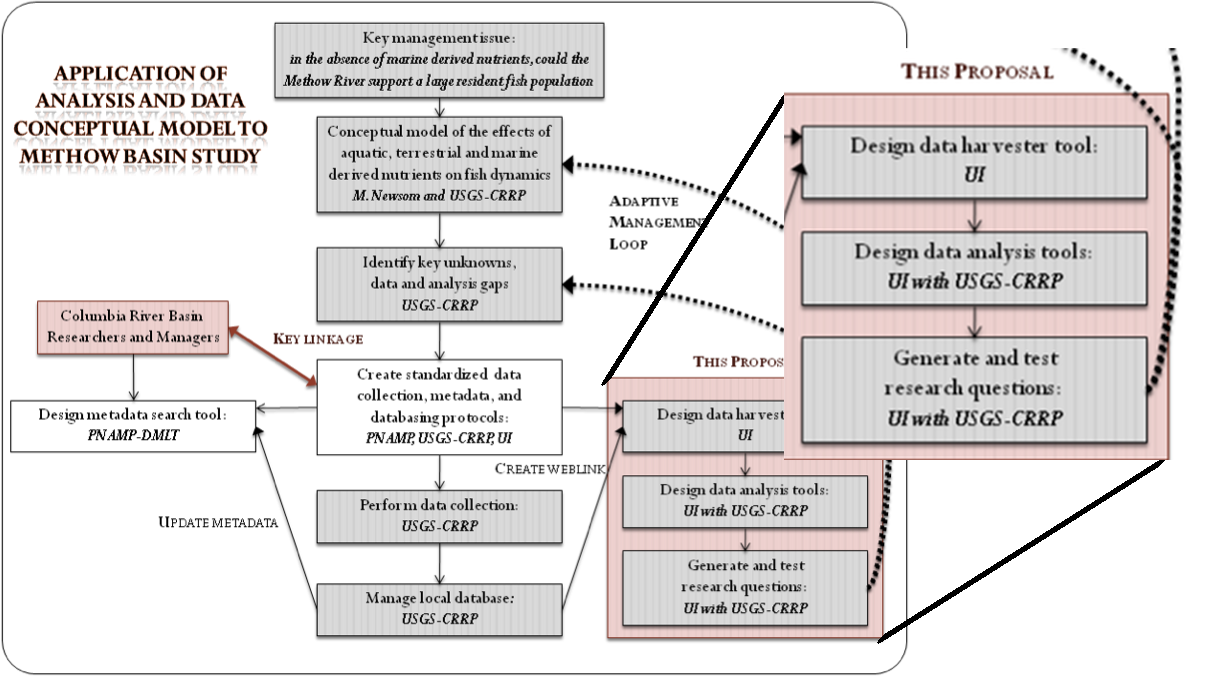
\includegraphics[width=120mm]{images/combo_proposal}
                \caption{This proposal software's application domain in DE-CRRP}
                \label{combo_proposal}
        \end{center}
\end{figure}

The proposed project will implement the UI data harvester portion of the grant
funded USGS-CRRP project (Figure~\ref{combo_proposal}), directed by Alex
Fremier of the UI College of Natural Resources. The data management tool will
use a web-based GUI that can be installed locally on the clients' computers,
but may also be accessed remotely.  The tool will contain a expandable meta
data server that can be connected to others to form a replicated data storage
system. It will use an existing RESTful networking protocol that will allow for many
different data formats to be synchronized across the cloud. The project will
also have a graphical, web-based interface for simplified data management.

The replicated in-cloud model allows some significant advantages to
researchers.  They can see exactly what their data looks like before they
submit it, due to the integrated visualizations.  They can filter out bad data
before it consumes bandwidth, and can retract undesirable data from the cloud,
even after synchronizing it. It also frees them from central storage service
management and fees, and encourages internode and inter-research communication.
The tool can be set up on multiple hosts, and can be used for the benefits of
the centralized cloud model. Each client can decide what topology suites them
best.

This model uses a distributed database model.
Distributed databases increase availability and reliability through automatic
replication. They are more
easily expandable, and can better protect from data loss from local disasters or
malicious attacks. Moving data to where it is in highest demand also increases
query performance. Offloading archive data to remote site with more 
resources preserves local resources. Replicated datasets can guarantee 
better availability. By staging data locally and filtering it before allowing
it to be exchanged, the autonomy of the organization is better preserved, and the
relevance of uploaded data can be improved. 

%probably some specific network protocols, like SOAP, etc, should be mentioned
%Alex, the network protocol doesn't have to apply just to low bandwidth users
%, but also to large data transfers
The network protocol will allow incremental synchronization of data from host
to host, even in less reliable environments. The tool will create
an outreach from researchers in high availability areas to those
in low availability, low bandwidth areas, and back. The network protocol
will have support for major data formats such as CSV, and allow
users to send incremental pieces of the data.

The intuitive interface will allow users to sort and manipulate their data,
needing only basic knowledge of computers (and naturally, the data in
question). Simple queries will create data subsets that users can bring to
a workspace. The tool will be able to sort data however the user likes, on the
fly. It will then be able to graph the ranges in the subset in most ways the
user could want to sort them.

Once the user has manipulated their data subset to their satisfaction, they
will be able to save instantly on the server and download it as a CSV file. The
tool will also be extensible so that future analysis modules will allow them to
run analysis on the local host, or remotely. These modules will be capable of
running analysis jobs on other designated compute hosts, like workstations,
clusters, or even Amazon's EC2. The tool will come only with basic
functionality for local analysis modules, but will be extensible for future, heavier
compute options.
%\required{Intellectual Merit} This is why your project is interesting and will
%help further knowledge in the field of mathematics. 

%\required{Broader Impacts}
% There are 4 kinds of broader impacts.
% 1. advance discovery and understanding while promoting teaching,
% training and learning
% 2. broaden the participation of underrepresented groups
% 3. disseminated broadly to enhance scientific and technological
% understanding
% 4. benefits of the proposed activity to society

